% !TEX TS-program = pdflatex
% !TEX encoding = UTF-8 Unicode

% This is a simple template for a LaTeX document using the "article" class.
% See "book", "report", "letter" for other types of document.

\documentclass[11pt]{article} % use larger type; default would be 10pt

\usepackage[utf8]{inputenc} % set input encoding (not needed with XeLaTeX)

%%% PAGE DIMENSIONS
\usepackage{geometry} % to change the page dimensions
\geometry{a4paper} % or letterpaper (US) or a5paper or....

\usepackage{graphicx} % support the \includegraphics command and options

\usepackage{amssymb}
\usepackage{amsmath}
%%% PACKAGES
\usepackage{booktabs} % for much better looking tables
\usepackage{array} % for better arrays (eg matrices) in maths
\usepackage{paralist} % very flexible & customisable lists (eg. enumerate/itemize, etc.)
\usepackage{verbatim} % adds environment for commenting out blocks of text & for better verbatim
\usepackage{subfig} % make it possible to include more than one captioned figure/table in a single float
% These packages are all incorporated in the memoir class to one degree or another...

%%% HEADERS & FOOTERS
\usepackage{fancyhdr} % This should be set AFTER setting up the page geometry
\pagestyle{fancy} % options: empty , plain , fancy
\renewcommand{\headrulewidth}{0pt} % customise the layout...
\lhead{}\chead{}\rhead{}
\lfoot{}\cfoot{\thepage}\rfoot{}

%%% SECTION TITLE APPEARANCE
\usepackage{sectsty}
\allsectionsfont{\sffamily\mdseries\upshape} % (See the fntguide.pdf for font help)
% (This matches ConTeXt defaults)

%%% ToC (table of contents) APPEARANCE
\usepackage[nottoc,notlof,notlot]{tocbibind} % Put the bibliography in the ToC
\usepackage[titles,subfigure]{tocloft} % Alter the style of the Table of Contents
\renewcommand{\cftsecfont}{\rmfamily\mdseries\upshape}
\renewcommand{\cftsecpagefont}{\rmfamily\mdseries\upshape} % No bold!
\usepackage{graphicx}
\graphicspath{ {./pings/} }

\usepackage{amsmath}
\DeclareMathOperator*{\argmax}{arg\,max}
\DeclareMathOperator*{\argmin}{arg\,min}

\newcount\colveccount
\newcommand*\colvec[1]{
        \global\colveccount#1
        \begin{pmatrix}
        \colvecnext
}
\def\colvecnext#1{
        #1
        \global\advance\colveccount-1
        \ifnum\colveccount>0
                \\
                \expandafter\colvecnext
        \else
                \end{pmatrix}
        \fi
}

%%% END Article customizations

%%% The "real" document content comes below...

\title{Macro PS3}
\author{Michael B. Nattinger\footnote{I worked on this assignment with my study group: Alex von Hafften, Andrew Smith, and Ryan Mather. I have also discussed problem(s) with Emily Case, Sarah Bass, and Danny Edgel.}}

%\date{} % Activate to display a given date or no date (if empty),
         % otherwise the current date is printed 

\begin{document}
\maketitle
\section{Question 1}
We will construct the sequential market structure equilibrium. Each period, we our bond markets contain claims to each "tree". 
\subsection{Part A}
Define $q_t^i$ as the price in period $t$ of a consumption good in period $t+1$ on the condition that consumer $i$ receives an endowment in period $t+1$. $b_t^{i,j}$ is the quantity of that bond demanded by person $j$.

Each agent maximizes expected utility:
\begin{align}
\max_{\{c_t^1,b_t^{1,1},b_t^{2,1}\}_{t=0}^{\infty}} E_0 \sum_{t=0}^{\infty}\beta^tlog c_t^1 \label{eqn:opt1}
\end{align}
\begin{align*}
\text{s.t. } c_t^1 + q_t^1b_t^{1,1} + q_t^2b_t^{2,1} \leq e_t^1 + b_{t-1}^{1,1}1\{ e_t^1=1 \} +  b_{t-1}^{2,1}1\{ e_t^2=1 \} %note: can rewrite indicators as just e from inside the indicator
\end{align*}
\begin{align}
\max_{\{c_t^2,b_t^{1,2},b_t^{2,2}\}_{t=0}^{\infty}} E_0 \sum_{t=0}^{\infty}\beta^tlog c_t^2 \label{eqn:opt2} 
\end{align}
\begin{align*}
\text{s.t. } c_t^2 + q_t^1b_t^{1,2} + q_t^2b_t^{2,2} \leq e_t^2 + b_{t-1}^{1,2}1\{ e_t^1=1 \} +  b_{t-1}^{2,2}1\{ e_t^2=1 \} 
\end{align*}

Market clearing implies the following conditions:
\begin{align}
b_t ^{1,1} + b_t^{1,2} &= 0 \label{eqn:mktcl1} \\
b_t ^{2,1} + b_t^{2,2} &= 0 \label{eqn:mktcl2} \\
c_t^1+c_t^2 &= e_t^1 + e_t^2 \label{eqn:mktcl3}
\end{align}

The competitive equilibrium is a set of prices $\{ q_t^1,q_t^2 \}_{t=0}^{\infty}$ and allocations $\{ b_t^{1,1},b_t^{2,1}, b_t^{1,2},b_t^{2,2},c_t^1,c_t^2\}_{t=0}^{\infty}$ such that agents optimize (\ref{eqn:opt1}),(\ref{eqn:opt2}) and markets clear (\ref{eqn:mktcl1}),(\ref{eqn:mktcl2}),(\ref{eqn:mktcl3}).

\subsection{Part B}
Our bellman equation for state $t<s$ takes the following form:
%V(b_t^)

Once the future endowment has shifted, it will remain shifted forever. So, after state $s$, no agent will buy assets to claims which pay out in the non-shifted state of next period. So, this value function for individual 1,2 takes the following form: 

\begin{align}
V_{2,1}((b)^{2,1}) &= \max_{(b')^{2,1}} log((b)^{2,1} - q^2(b')^{2,1}) + \beta V_{2,1}((b')^{2,1}) \label{eqn:v21}
\end{align}

\begin{align}
V_{2,2}(b^{2,2}) &= \max_{(b')^{2,2}} log(b^{2,2} - q^2(b')^{2,2} + 1) + \beta V_{2,2}((b')^{2,2})  \label{eqn:v22}
\end{align}

Pre-shift, our value functions are of the following form:

\begin{align}
V_{1,1}((b)^{1,1}) &= \max_{(b')^{1,1},(b')^{2,1}} log(1+(b)^{1,1} - q^1(b')^{1,1}  - q^2(b')^{2,1}) + \beta ((1-\delta)V_{1,1}((b')^{1,1}) + \delta V_{2,1}((b')^{2,1}))  \label{eqn:v11}
\end{align}

\begin{align}
V_{1,2}(b^{1,2}) &= \max_{(b')^{1,2},(b')^{2,2}} log(b^{1,2} - q^1(b')^{1,2}-  q^2(b')^{2,2}) + \beta  ((1-\delta)V_{1,2}((b')^{1,2}) + \delta V_{2,2}((b')^{2,2}))  \label{eqn:v12}
\end{align}

We must solve backwards, so first we will solve eqns (\ref{eqn:v21}),(\ref{eqn:v22}) by taking first order conditions and envelope conditions:
\begin{align*}
\frac{q^2}{(b)^{2,1} - q^2(b')^{2,1}} &= \beta V'_{2,1}((b')^{2,1})\\
V'_{2,1}((b)^{2,1})&= \frac{1}{(b)^{2,1} - q^2(b')^{2,1}}\\
\Rightarrow q^2(c')^{2,1} &= \beta c^{2,1},\\
\frac{q^2}{(b)^{2,2} - q^2(b')^{2,2} + 1} &= \beta V'_{2,1}((b')^{2,2})\\
V'_{2,2}((b)^{2,2})&= \frac{1}{(b)^{2,2} - q^2(b')^{2,2}+1}\\
\Rightarrow q^2(c')^{2,2} &= \beta c^{2,2}.
\end{align*}

From our market clearing condition (\ref{eqn:mktcl3})%,(\ref{eqn:mktcl3}) we have:
\begin{align*}
(c)^{2,1} + (c)^{2,2} &= 1 = (c')^{2,1} + (c')^{2,2}\\
\Rightarrow (c)^{2,1} + (c)^{2,2} &= \frac{\beta}{q^2}((c)^{2,1} + (c)^{2,2})\\
%\Rightarrow (c)^{2,2}&= 1 -  (c)^{2,1}\\
%b^{2,1} + b^{2,2 } &=0\\
%(c)^{2,1} &=  (b)^{2,1} - q^2(b')^{2,1} \\
%&=  (b)^{2,1} + q^2(b')^{2,1}\\
\end{align*}
\begin{align}
\Rightarrow q^2 &=\beta, \\
\Rightarrow c^{2,1}&=(c')^{2,1},\\
\Rightarrow c^{2,2}&=(c')^{2,2}
\end{align}
after the switch.

Now we can take FOCs and envelope conditions of  (\ref{eqn:v11}),(\ref{eqn:v12})
\begin{align*}
\frac{q^1}{1+b^{1,1} - q^1(b')^{1,1}-  q^2(b')^{2,1}} &= \beta(1-\delta)V'_{1,1}((b')^{1,1})\\
V'_{1,1}((b)^{1,1})&=\frac{1}{1+b^{1,1} - q^1(b')^{1,1}-  q^2(b')^{2,1}}\\
\Rightarrow \frac{(c')^{1,1}}{(c)^{1,1}}&= \frac{\beta(1-\delta)}{q^1},\\
\frac{q^2}{1+b^{1,1} - q^1(b')^{1,1}-  q^2(b')^{2,1}} &= \beta\delta V'_{2,1}((b')^{2,1})\\
\Rightarrow \frac{ (c')^{2,1}}{(c)^{1,1}} &= \frac{\beta\delta}{q^2},\\
\frac{q^1}{b^{1,2} - q^1(b')^{1,2}-  q^2(b')^{2,2}} &= \beta(1-\delta)V'_{1,2}((b')^{1,2})\\
V'_{1,2}((b)^{1,2})&=\frac{1}{b^{1,2} - q^1(b')^{1,2}-  q^2(b')^{2,2}}\\
\Rightarrow \frac{(c')^{1,2}}{(c)^{1,2}}&= \frac{\beta(1-\delta)}{q^1},\\
\frac{q^2}{b^{1,2} - q^1(b')^{1,2}-  q^2(b')^{2,2}} &= \beta\delta V'_{2,2}((b')^{2,2})\\
\Rightarrow \frac{ (c')^{2,2}}{(c)^{1,2}} &= \frac{\beta\delta}{q^2}
\end{align*}

From the above set of equations the following set of identities are easily derived:
\begin{align}
 \frac{(c')^{1,1}}{(c)^{1,1}}&=\frac{\beta(1-\delta)}{q^1} =  \frac{(c')^{1,2}}{(c)^{1,2}}\\
\frac{ (c')^{2,1}}{(c)^{1,1}} &= \frac{\beta\delta}{q^2} = \frac{ (c')^{2,2}}{(c)^{1,2}}
\end{align}

We can now combine with our market clearing condition  (\ref{eqn:mktcl3}) and find:

\begin{align*}
(c)^{1,1} + (c)^{1,2} &= 1 = (c')^{1,1} + (c')^{1,2}\\
&= \frac{\beta(1-\delta)}{q^1}((c)^{1,1} + (c)^{1,2})\\
\Rightarrow q^1 &= \beta(1-\delta),\\
(c)^{1,1} + (c)^{1,2} &= 1 = (c')^{2,1} + (c')^{2,2}\\
&=  \frac{\beta\delta}{q^2}((c)^{1,1} + (c)^{1,2})\\
\Rightarrow q^2 &= \beta \delta
\end{align*}

Now we will solve for the consumption allocations.

The first-type consumer brings in $b_{s-1}^{2,1}$ into the post-shift period. They will consume a constant amount each period, and the first-type consumer will also consume a constant amount each period. Thus, we know that $b^{2,1}_{s+t} = b_{s-1}^{2,1}, b^{2,2}_{s+t} = b_{s-1}^{2,2} \forall t\geq0$, as they can afford to do so and consuming a lesser amount each period would be non-optimal, and consuming more is not affordable. The first-type consumer, therefore, buys $b_{s-1}^{2,1}$ bonds in each period at price $q^2 = \beta$ from their period budget of $b_{s-1}^{2,1}$ and therefore has $(1-\beta)b_{s-1}^{2,1}$ value left to consume, which they will in each period. Therefore, $c_t^{2,1} = (1-\beta)b_{s-1}^{2,1} \forall t\geq s$ and from our market clearing condition we know that $c_t^{2,2} = 1-((1-\beta)b_{s-1}^{2,1}) \forall t\geq s.$  

Now we can look forward.

\begin{align*}
c^{1,2} &= (c')^{2,2}\\
&=  1-((1-\beta)b_{s-1}^{2,1})\\
c^{1,1} &= (c')^{2,1}\\
&= (1-\beta)b_{s-1}^{2,1}
\end{align*}
So, consumption will be constant for each consumer across periods. We know that the consumption will be the highest level such that this can be maintained, so contingent bond claims will remain constant over time or else either the consumers are not optimizing consumption (if bond claims are exploding) or the consumption levels cannot be afforded (if the bond claims are falling to 0). Now we just need to solve for the values by computing the budget constraints:

\begin{align*}
1+b^{1,1}&= c^{1,1} + q^1b^{1,1} + q^2b^{2,1}\\
&=  (1-\beta)b^{2,1} + \beta(1-\delta)b^{1,1} +  \beta \delta b^{2,1} \\
\Rightarrow 1+(1-\beta + \beta \delta)b^{1,1} &= (1-\beta+\beta\delta)b^{2,1}\\
\Rightarrow b^{1,1}  &=  b^{2,1}+\frac{-1}{1-\beta + \beta \delta}
%b^{2,1}&=c^{2,1}
%b^{1,2} &=  c^{1,2} + q^1b^{1,2} + q^2b^{2,2}\\
%\Rightarrow -b^{1,1} &=  1-((1-\beta)b^{2,1}) - \beta(1-\delta)b^{1,1} -  \beta \delta b^{2,1} 
%1+b^{2,2}&= c^{2,2} + q^2 b^{2,2} \\
%1-b^{2,1}&= 1-((1-\beta)b^{2,1}) - \beta b^{2,1}
\end{align*}


In the first period, the first-type consumer has only the unit endowment with which they can purchase the first allocation of bonds:

\begin{align*}
1 &= c^{1,1} + q^1b^{1,1} + q^2b^{2,1}\\
 &= (1-\beta)b^{2,1} + ( \beta(1-\delta))\left( b^{2,1}+\frac{-1}{1-\beta + \beta \delta}\right) + (\beta\delta)b^{2,1}\\
\Rightarrow  b^{2,1} &= 1 + \frac{\beta - \beta\delta}{1-\beta + \beta\delta}\\
&= \frac{1}{1-\beta + \beta\delta}. 
\end{align*}
Therefore, our consumption allocations are $c^{1,1} = c^{2,1} = \frac{1-\beta}{1-\beta + \beta\delta}$, $c^{1,2} = c^{2,2} = \frac{\beta\delta}{1-\beta + \beta\delta}.$
\subsection{Part C}

We solved in part C for the price of a claim to the consumption good: prior to the switch, the price of a claim to the consumption allocation is  $q^1+q^2 = \beta $ and after the switch the price of a claim to the consumption allocation is $q^2 = \beta$.

Prior to the switch, we can construct a risk-free bond yielding one unit of consumption by purchasing one bond which pays one unit of consumption in each of the two possible futures: $q^f = q^1 + q^2 = \beta$. Similarly, after the swap we can buy a claim of the 2-type bond, $q^f = q^2 = \beta$. Therefore, in either case the price of a risk-free bond is $\beta$, so for $\beta = \frac{1}{1+R^f} \Rightarrow R^f = \frac{1}{\beta} -1$.
\subsection{Part D}
The social planner problem becomes the following:
\begin{align*}
\max_{c_t}E\left[ \sum_{t=0}^{\infty} \beta^t u_{\lambda}(c_t) \right]\\
\text{s.t. } c^{1}_t + c^{2}_t = 1 \\
\text{where } u_{\lambda}(c_t) = \max_{c_t^1,c_t^2} \lambda log(c_t^1) + (1-\lambda)log(c_t^2)\\
\text{s.t.} c_t^1+ c_t^2 = c_t
\end{align*}
Since our total allocation of consumption goods is 1 in all periods, our social planner's problem is really just solving the subproblem
\begin{align*}
&\max_{c_t^1,c_t^2} \lambda log(c_t^1) + (1-\lambda)log(c_t^2) \\
&\text{s.t.} c_t^1+ c_t^2 = 1\\
\Rightarrow  &\max_{c_t^1} \lambda log(c_t^1) + (1-\lambda)log(1-c_t^1) \\
\Rightarrow &\frac{\lambda}{c_t^1} = \frac{1-\lambda}{1-c_t^1} \\
\Rightarrow &\lambda - \lambda c_t^1 = c_t^1 - \lambda c_t^1\\
\Rightarrow &c_t^1 = \lambda\\
\Rightarrow &c_t^2 = 1-\lambda
\end{align*}
\subsection{Part E}
For $\lambda = \frac{1-\beta}{1-\beta + \beta\delta}$, the competitive equilibrium is optimal. Given $\lambda$, we would be able to decentralize the pareto optimum as a competitive equilibrium by setting the type-1 individual allocation in the first period to be a particular value which we can solve for below.

Let the first period allocation of the type-1 person be $w$ and fix $\lambda$ as the pareto weight.

As in part B we can solve the initial-period allocation and find an expression for the type-1 individual's consumption as a function of $w$:

\begin{align*}
w &= c^{1,1} + q^1b^{1,1} + q^2b^{2,1}\\
 &= (1-\beta)b^{2,1} + ( \beta(1-\delta))\left( b^{2,1}+\frac{-1}{1-\beta + \beta \delta}\right) + (\beta\delta)b^{2,1}\\
\Rightarrow  b^{2,1} &= w + \frac{\beta - \beta\delta}{1-\beta + \beta\delta}\\
 \Rightarrow c^{1,1} = c^{2,1} = \lambda &= (1-\beta)\left( w + \frac{\beta - \beta\delta}{1-\beta + \beta\delta}\right)\\
\Rightarrow w &= \frac{\lambda}{1-\beta} -  \frac{\beta - \beta\delta}{1-\beta + \beta\delta}
\end{align*}

So, if the social planner replaces the type-1 individual's first-period endowment with $w = \frac{\lambda}{1-\beta} -  \frac{\beta - \beta\delta}{1-\beta + \beta\delta}$, then the pareto-optimal allocation will be achieved by the competitive equilibrium.

\section{Question 2}
\subsection{Part A}
\subsection{Part B}
\subsection{Part C}
\subsection{Part D}
\section{Question 3}
\subsection{Part A}
Our bellman equation takes the following form:

\begin{align*}
V(a,l) &= \max_{a'} \frac{(wl +(1+r)a - a')^{1-\gamma}}{1-\gamma} + \beta E[V(a',l')]\\
&=  \max_{a'} \frac{(wl +(1+r)a - a')^{1-\gamma}}{1-\gamma} + \beta (V(a',l_h)P(l'=l_h|l) + V(a',l_h)P(l'=l_h|l))
\end{align*}
Taking FOCs and applying the envelope conditions,
\begin{align*}
(wl +(1+r)a - a')^{-\gamma} &= \beta(V'(a',l_h)P(l'=l_h|l) + V'(a',l_h)P(l'=l_h|l))\\
V'(a,l) &= (1+r)(wl +(1+r)a - a')^{-\gamma}\\
\Rightarrow c^{-\gamma} &= \beta(1+r)((c'_h)^{-\gamma}P(l'=l_h|l) + (c'_l)^{-\gamma}P(l'=l_h|l) )
\end{align*}
The above equation forms our optimality conditions.
\subsection{Part B}
In the stationary distribution, $PQ = P$ where $P = [P_l P_h]$. We can easily solve for this distribution numerically from an arbitrary starting point. As this is a very simple markov process, markov-chain monte carlo methods will converge to the stationary distribution by standard ergodic properties which $Q$ easily satisfies. We can therefore start with an arbitrary initial distribution $P_0$ and iterate through the transition matrix $Q$, with product $P:=P_0Q$ becoming next iteration's $P_0$, until $P$ and $P_0$ have converged to some tolerance. 

The numerical solution is $P = [0.25 0.75] $ so the stationary distribution has $3/4 $ of the weight on the high-labor distribution, and the rest on the low-labor distribution. Therefore, the unconditional mean of the labor endowment is $0.25(0.7) + 0.75(1.1) = 1$.

\subsection{Part C}
I solved for the value function numerically. Results are plotted below.

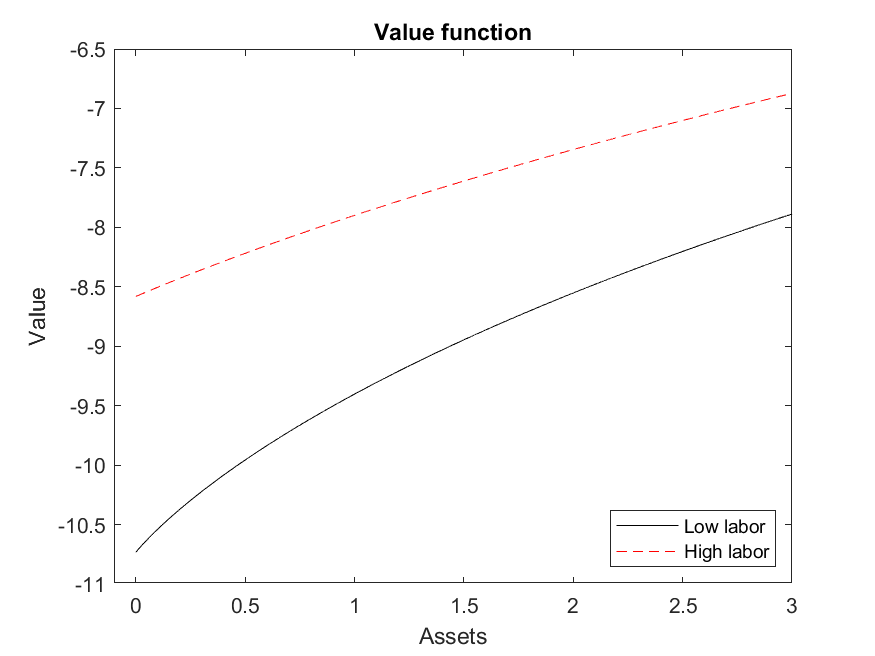
\includegraphics{valfunc}

The value function solution does appear to be continuous, increasing, concave, and differentiable. The value from having a high labor draw is higher than the value from having a low labor draw. All of these features are as predicted by theory.

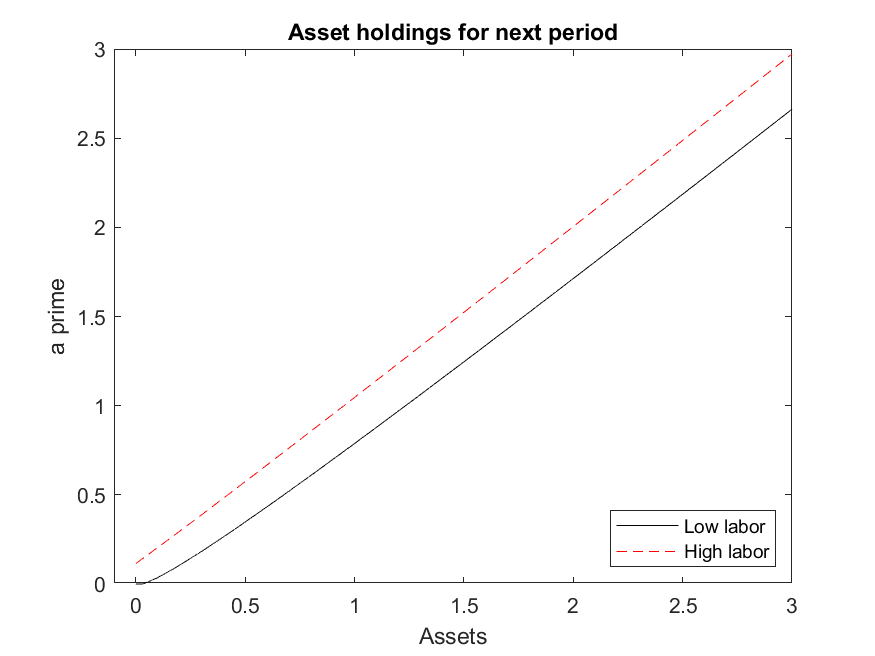
\includegraphics{aprime}

Above we see the asset holding decision rules for the two labor shocks. We can see the value $\bar{a}$ such that $a'<a \forall a\geq \bar{a}$ on the graph that follows.

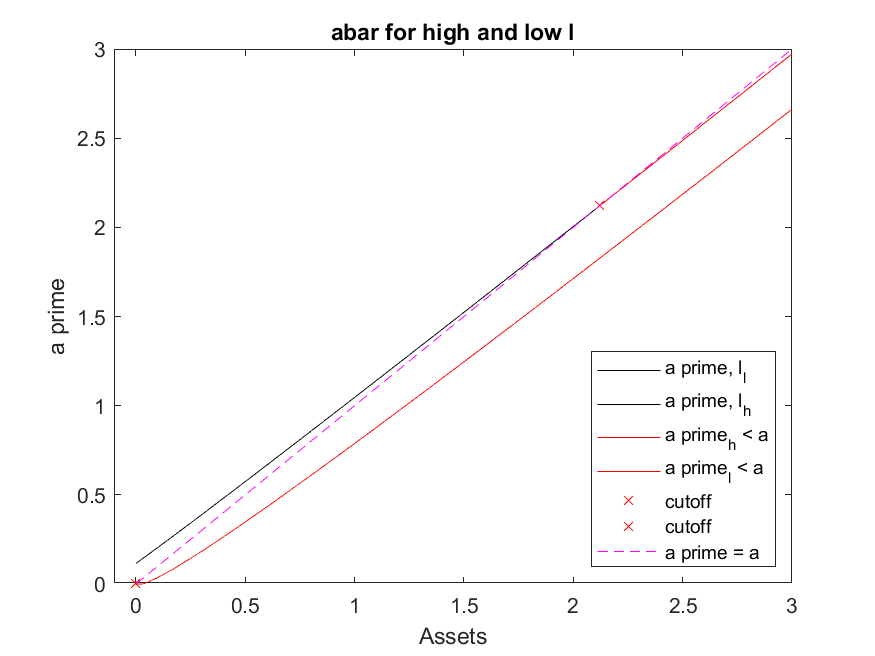
\includegraphics{abar}

Above we see the value $\bar{a}$ such that $a'<a \forall a\geq \bar{a}$. This exists for both the high and low labor shocks which means that our assumption that asset holdings can be restricted to a convex set is validated. Furthermore, we can see that all asset levels will result in running down assets if one receives a low labor level. This implies a unit mass of asset holdings at 0.

\subsection{Part D}

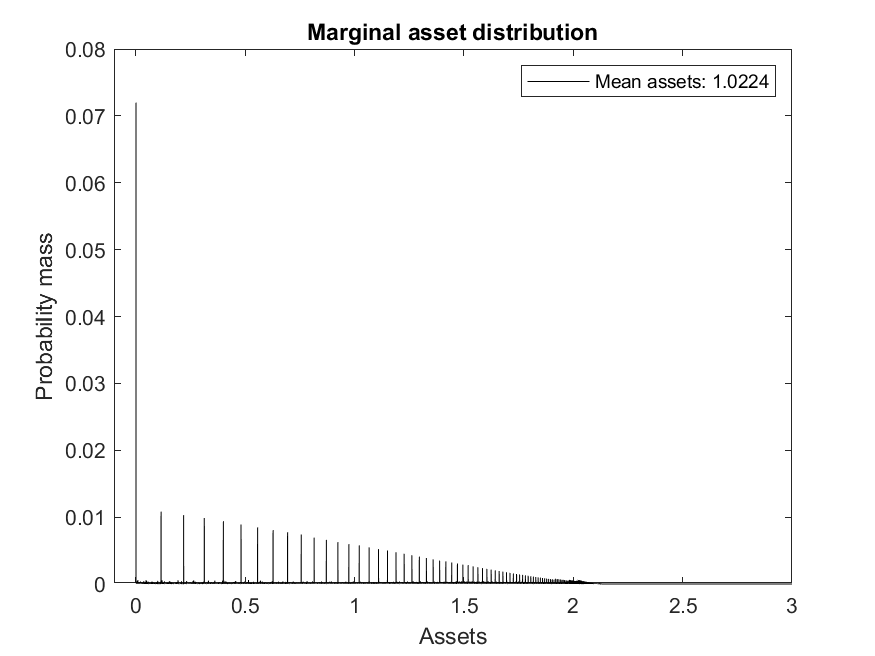
\includegraphics{marginal}

Above we see the marginal asset distribution. It has some interesting features. First, it has a large mass at $0$. This is because drawing a low labor level at a low asset position results in no savings so there is a large proportion of individuals that end up having no savings. Next we can see ridges of high density pop up at regular intervals. Each such ridge represents the savings of those that were at the previous ridge in the previous turn, and received a high labor draw, with the first ridge being asset savings of 0. In other words, the first large mass is at 0, the second mass is the proportion of those in in the fist mass that receive a high labor draw, the third mass is the proportion of those in the second mass that receive a high labor draw, and so on.
\end{document}
